\PassOptionsToPackage{top=3cm,left=3cm,right=3cm,bottom=3cm}{geometry}
\documentclass[fleqn,11pt]{wlscirep}

\usepackage{import}
\usepackage{../paper/main-lancet}

\renewcommand{\paragraph}[1]{\vspace{0.3cm}\noindent\underline{\emph{#1}}\hfill\noindent}

\begin{document}

\doublespacing

\title{\bfseries\LARGE\singlespacing{Brief report:
Molecular detection of SARS-CoV-2 and other respiratory viruses in saliva and bioaerosols}}

% author list
\author[1,2]{Nicolas Banholzer}
\author[2,3]{Philipp Jent}
\author[2,4]{Pascal Bittel}
\author[1]{Kathrin Zürcher}
\author[4]{Lavinia Furrer}
\author[1]{Simon Bertschinger}
\author[5]{Ernest Weingartner}
\author[2,4]{Alban Ramette}
\author[1,6,7]{Matthias Egger}
\author[2,8]{Tina Hascher}
\author[1*,2]{Lukas Fenner}

\affil[1]{Institute of Social and Preventive Medicine, University of Bern, Bern, Switzerland}
\affil[2]{Multidisciplinary Center for Infectious Diseases, University of Bern, Bern, Switzerland}
\affil[3]{Department of Infectious Diseases, Inselspital, Bern University Hospital, University of Bern, Bern, Switzerland}
\affil[4]{Institute for Infectious Diseases, University of Bern, Bern, Switzerland}
\affil[5]{Institute for Sensors and Electronics, University of Applied Sciences and Arts Northwestern Switzerland, Windisch, Switzerland}
\affil[6]{Population Health Sciences, University of Bristol, Bristol, UK}
\affil[7]{Centre for Infectious Disease Epidemiology and Research, University of Cape Town, Cape Town, South Africa}
\affil[8]{Institute of Educational Science, University of Bern, Bern, Switzerland}

\affil[*]{Corresponding author: lukas.fenner@unibe.ch}


\vspace{2em}

%TC:ignore

\begin{information}\normalfont
\textbf{Word count:} Abstract 150 (max 150), Manuscript 1,625 (max 1,500) \\
\textbf{Display items:} Figure 1 \\
\textbf{References:} 17 (max 12) \\
%\textbf{Supporting information:} STROBE checklist, Supplementary Data with texts, tables, and figures
% \par
\end{information}

\begin{abstract}\normalfont
\noindent We compared airborne and saliva samples from two studies conducted in winter 2021/2022 (during the SARS-CoV-2 omicron wave) and winter 2022/2023 (after the COVID-19 pandemic) in a Swiss school setting. While during the pandemic we detected almost exclusively SARS-CoV-2 in saliva (19~samples of SARS-CoV-2 vs 2~samples of non-SARS-CoV-2), after the pandemic the most common respiratory viruses were adenovirus, influenza, and rhinoviruses (3~samples of SARS-CoV-2 vs 47~samples of non-SARS-CoV-2). Despite the same study setting and methods used, airborne detection of SARS-CoV-2 was relatively more frequent than of non-SARS-CoV-2 viruses (10~samples of SARS-CoV-2 in 2021/2022 vs 2~samples of non-SARS-CoV-2 in 2022/2023). SARS-CoV-2 was also detected more frequently on the HEPA-filters of installed portable air cleaners (6~samples of SARS-CoV-2 vs 3~samples of non-SARS-CoV-2). Our comparison suggests that SARS-CoV-2 is easier to detect in the air than other endemic respiratory viruses, possibly facilitating long-range transmission. \medskip

\par
\end{abstract}

\flushbottom
\maketitle

\vspace{2em}

\vspace{0.5em}

\noindent\textbf{Keywords:} respiratory viruses; SARS-CoV-2; influenza; airborne transmission; molecular detection
% maximum of 3-5 keywords

\thispagestyle{empty}
\sloppy
\raggedbottom

\newpage
%TC:endignore

\setcounter{page}{1}

\section*{Introduction}

The transmission of respiratory viruses, such as SARS-CoV-2 and influenza, within schools and and other indoor environments is difficult to control\cite{Leung2020}. Respiratory viruses spread by multiple routes, including respiratory particles such as large droplets and small aerosols. Unlike larger droplets, which settle quickly, aerosols can remain suspended in the air for extended periods\cite{Wang2021}. Airborne transmission is probably significant, but the relative contribution to overall transmission is still unclear, particularly because detection of respiratory viruses in the air remains challenging\cite{Belser2023PLOSPath}.

Airborne infectious pathogens are primarily found in smaller particles (<10$\mu$m) and the distribution is similar across a range of different pathogens\cite{Fennelly2020}. Thus, pathogen-carrying aerosols have the potential for long-range transmission, but the larger concentration of particles near the infectious person favours short-range transmission\cite{Tellier2009JTRSI,Wang2020}. The complexity of airborne transmission lies in the interplay between the physicochemical properties of pathogen-carrying aerosols and environmental conditions\cite{Wang2021}, making it challenging to devise effective public health strategies to mitigate the spread of respiratory infections in various indoor settings, including schools, offices, and hospitals.

In this study, we compared saliva samples, bioaerosol samples, and samples from the HEPA filters of air cleaners that were collected as part of two studies that we conducted in a Swiss school setting in winter 2021/2022 (during the SARS-CoV-2 omicron wave, henceforth 2022)\cite{Banholzer2023PLoSMed} and winter 2022/2023 (after the COVID-19 pandemic, henceforth 2023)\cite{Banholzer2023submitted}. We show differences in the distribution of respiratory viruses and analyze the results from airborne molecular detection. 


\section*{Methods}

Data was collected in Swiss secondary schools (age of students 14-17~years) in the canton of Solothurn, Switzerland, over a seven-week study period from end of January to beginning of March. Two classes of two different secondary schools (school 1 and 2) participated in 2022 and two classrooms of one secondary school (\ie only school 2) participated in 2023. In 2022, a general mask mandate was in place for the first 3~study weeks, followed by 2~weeks without intervention, and another 2~weeks during which air cleaners were installed in the classrooms. In 2023, air cleaners were installed for half of the study period in the classrooms following a cross-over study design. 

All classrooms were not equipped with an active HVAC (heating, ventilation, air conditioning) system, but were ventilated using passive window ventilation. An air quality device (AQ Guard, Palas GmbH, Karlsruhe, Germany) continuously measured indoor CO$_2$ levels, temperature, and humidity. In 2022, passive window ventilation occurred per recommendations of the national public health authorities. In school~1, ventilation was additionally assisted by a CO$_2$ guided opener of a small window at the top. In 2023, passive window ventilation occurred solely at the discretion of the teachers. 

Receptive testing for a panel of respiratory infections was done weekly in 2022 and bi-weekly in 2023. Airborne respiratory viruses were collected in each classroom with a cyclonic bioaerosol sampling device (Coriolis Micro Air, Bertin Instruments Montigny-le-Bretonneux, France) and a BioSpot-VIVAS condensation particle growth collection device (Aerosol Devices Inc., Ft. Collins, CO, USA)\cite{Lednicky2016AST}. The removable parts were regularly autoclaved. Finally, swabs from the air cleaners' HEPA filters were collected at the end of the study in 2022 and after each intervention phase in 2023. The HEPA filters were removed and divided into 20~fields. One sterile Phosphate-Buffered Saline-moistened swab per field was then taken for a total of 20~swabs per filter. Saliva and airborne samples were transported to the Institute of Infectious Diseases and stored at $-$80°C until further processing\cite{Huber2021}. 

Prior to the real-time (RT)-PCR analysis, daily bioaerosol samples were combined for each sampling device and filtered using Amicon Ultra-15 Centrifugal Filters with Ultracel 10,000 Dalton molecular weight cutoffs filters (UFC9010; MilliporeSigma, Burlington, USA) to a volume of 1\,mL. Saliva samples were analyzed directly without prior filtration. The Allplex RV Master Assay (Seegene, Seoul, South Korea) detects a panel of 19 major respiratory viruses and viral subtypes, including SARS-CoV-2, influenza A/B, respiratory syncytial, metapneumovirus, adenovirus, rhinovirus, and parainfluenza. 

Descriptive statistics were used to present differences in the type, number, and proportion of respiratory viruses detected in saliva and airborne samples between 2022 and 2023.

\section*{Results}

In 2022, 44~students participated in weekly saliva testing. There were 21~positive saliva samples over the study, namely 19~SARS-CoV-2, 1~influenza~A, and 1~adenovirus. There were 10~positive bioaerosol samples, namely 9~SARS-CoV-2 and 1~adenovirus. There were 8~positive samples on the HEPA-filters of the air cleaners, namely 6~SARS-CoV-2, 1~influenza~A and 1~adenovirus. In 2023, 38~students from two classes of secondary school~2 participated in bi-weekly saliva testing. There were 50~positive saliva samples over the study, namely 15~influenza~B, 15~rhinovirus, 14~adenovirus, 3~SARS-CoV-2, 2~metapneumovirus, 1~parainfluenza virus. There were 2~positive bioaerosol samples, namely 1~rhinovirus and 1~adenovirus. There were 4~positive samples on the HEPA-filters of the air cleaners, namely 1~influenza~B, 1~rhinovirus, 1~adenovirus, and 1~SARS-CoV-2. 

In comparison, there was a clear shift in the distribution of respiratory viruses from predominantly SARS-CoV-2 in 2022 to predominantly non-SARS-CoV-2 viruses in 2023 (\Cref{fig:comparison}a). Molecular detection also varied between the two years, especially for airborne samples (\Cref{fig:comparison}b). For saliva, 21 out of 262~samples were positive in 2022 compared to 50 out of 448~samples in 2023. For bioaerosols, 10 out of 130~samples were positive in winter 2022 compared to 2 out of 105~samples in 2023 . For the HEPA-filters, 8 out of 40~swabs were positive in 2022 compared to 4 out of 160~swabs in 2023. 

\begin{figure}
    \centering
    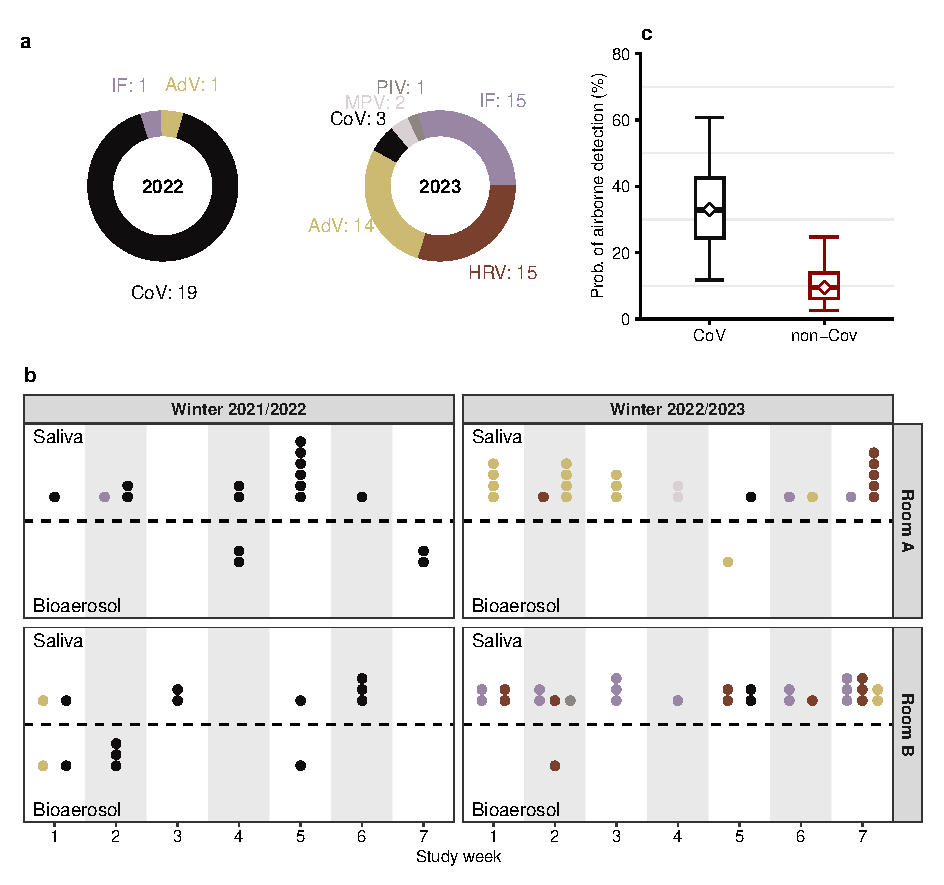
\includegraphics{results/comparison.pdf}
    \caption{Comparison of molecular detection of respiratory viruses between winter 2021/2022 (2022) and winter 2022/2023 (2023). \textbf{(a)}~Distribution of respiratory viruses found in saliva. IF: influenza~A/B, HRV: human rhinovirus, AdV: adenovirus, CoV: SARS-CoV-2, MPV: human metapneumovirus, PIV: parainfluenza virus. \textbf{(b)}~Number of positive samples in saliva, bioaerosols, and on the HEPA-filters of air cleaners.}
    \label{fig:comparison}
\end{figure}


Daily mean CO$_2$ level was 1,064\,ppm (standard deviation [SD] 232\,pppm) in 2022 compared to 1,702\,ppm (SD 370\,pppm) in 2023, suggesting that the classrooms were less well ventilated after the COVID-19 pandemic. Daily mean relative humidity was 38\% (SD 6\%) in 2022 compared to 38\% (SD 5\%) in 2023. Daily mean temperature was 19°C (SD 2°C) in 2022 compared to 22°C (SD 1°C) in 2023. 

\section*{Discussion}

We compared molecular data collected from two studies in Swiss secondary schools in winter 2021/2022 (2022) and 2022/2023 (2023). During the COVID-19 pandemic in 2022, we detected mainly SARS-CoV-2 in saliva and also in bioaerosols and on the HEPA-filters of air cleaners. After the pandemic in 2023, we detected a clear shift in the distribution of respiratory viruses towards mainly non-SARS-CoV-2 respiratory viruses such as influenza, adenovirus, and rhinovirus. These viruses were rarely detected in bioaerosols and on the HEPA-filters of air cleaners. 

The differences between the two study periods (pandemic versus non-pandemic) suggest that SARS-CoV-2 is easier to detect in the air. One possible explanation is that SARS-CoV-2 can remain suspended and active in the air for extended periods of time, facilitating long-range transmission. In contrast, non-SARS-CoV-2 viruses, such as influenza and adenovirus, were rarely detected in the air, suggesting they settle or become inactive more quickly, and require prolonged close contact for transmission. However, these findings should be interpreted with caution as they originate from an analysis of secondary data collected in a real-world setting, not a rigorous experiment. Furthermore, although there may be variations in the airborne survival of respiratory viruses, it is important to note that prolonged close contact continues to play a significant role in transmission. This holds true even for viruses capable of long-range transmission, as exemplified by SARS-CoV-2\cite{Leung2020NatMed,Lind2023NatCommun}.

Technical reasons for the differences in airborne detection are unlikely because the bioaerosol sampling devices and laboratory procedures were the same in both studies, and no technical problems were observed. Instead, airborne detection could have been influenced by environmental factors. Although temperature and relative humidity were similar in both study periods, the same levels may have different effects on the airborne survival of respiratory viruses\cite{Tellier2009JTRSI,Davis1971AM}. A change in ventilation conditions could also have had a profound effect, but CO$_2$ levels were even higher in winter 2023, suggesting that classrooms were not as well ventilated as during the COVID-19 pandemic. We speculate that the difference in airborne molecular detection is due to the different characteristics of the respiratory viruses. Differences in the physicochemical properties of virus-laden aerosols (\eg particle size and viral load), which influence the generation and survival of airborne viral RNA\cite{Wang2021}, may facilitate the detection of SARS-CoV-2 in the air. This is because viral loads often do not exceed the detection limits of existing devices for bioaerosol sampling, which remains a challenge\cite{Belser2023PLOSPath}. For example, one study failed to detect any human rhinovirus in the exhaled breath of 16~HRV-infected subjects\cite{Fabian2011JAMPDD}. However, several studies , including ours, have shown that sporadically non-SARS-CoV-2 viruses such as influenza, rhinovirus, and adenovirus can also be detected in the air\cite{Bischoff2013JID,Pan2017mSphere,Myatt2004AJRCCM}. Finally, the ability to detect pathogens in bioaerosols may be related to the patient characteristics of the study participants. Several studies have suggested an association between the generation of pathogenic aerosols and infectiousness\cite{Leung2020NatMed,Bischoff2013JID}. Therefore, studies that include more infectious patients (intentionally or unintentionally) are likely to have a higher chance of detecting respiratory viruses in the air. 

In conclusion, our comparison of two years of respiratory viral transmission in a school setting suggests that SARS-CoV-2 is easier to detect in indoor air as compared to other endemic viruses such as influenza, adenovirus and rhinoviruses. Future studies should test this hypothesis experimentally and investigate the relative importance of different modes of transmission.   

% We detected fewer respiratory viruses in bioaerosol samples compared to our previous study\cite{Banholzer2023PLoSMed} (1~sample of adenovirus and 1~sample of rhinovirus in this study vs 10~samples of SARS-CoV-2 in the previous study), especially in relation to the number of positive saliva samples (50~samples in this study vs 21~in the previous study). Similarly, the number of viruses detected on the filters of the air cleaners was also lower in this study (4~positive samples in 160~swabs vs 8~positive samples in 80~swabs in the previous study). Importantly,  in the current study compared to the previous study in 2022 during the SARS-CoV-2 Omicron variant. Whereas in 2022 we detected almost exclusively SARS-CoV-2 in human saliva, the most common respiratory viruses in 2023 were adenovirus, influenza~B, and rhinoviruses (only three SARS-CoV-2-positive samples). The shift in the pattern of respiratory viruses has been observed in other studies\cite{Nygaard2023Lancet,Sauteur2022EuroSurv}. 


\bibliography{references.bib}

\end{document}